\section{Definition of the signal region}
\label{sec:sigregion}

We define signal regions to look for possible
new physics contributions in the opposite sign isolated 
dilepton sample. The choice of signal region is driven by 
three observations:
\begin{enumerate}
\item astrophysical evidence for dark matter suggests that
we concentrate on the region of high \met;
\item new physics signals should have high $\sqrt{\hat{s}}$;
\item observable high cross section new physics signals 
are likely to be produced strongly;  thus, we expect significant
hadronic activity in conjunction with the two leptons.
\end{enumerate}

Following these observations, we define the following 3 signal regions ( shown
in figure ~\ref{fig:sigRegion} ) by adding requirements of large hadronic activity and missing
transverse energy to the preselection of Section~\ref{sec:eventSel}.
\begin{itemize}
\item 2010 signal region:       \Ht\ $>$ 300~GeV and $y > 8.5$~GeV$^{1/2}$.
\item high \met\ signal region: \Ht\ $>$ 300~GeV and \met\ $>$ 275 GeV
\item high \Ht\  signal region: \Ht\ $>$ 600~GeV and \met\ $>$ 200 GeV
\end{itemize}

In our 2010 analysis, we cut on the quantity $y \equiv \met/\sqrt{H_T}$ rather than \met\
because the variables \Ht\ and $y$ are
largely uncorrelated for the dominant $t\bar{t}$ background.  
This allows us to use a data-driven ABCD method to estimate the
background (see Section~\ref{sec:abcd}). Here, we include 2 additional tighter signal
regions using requirements on on \met\ and \Ht, since we observe that \met\ is a better 
discriminant between \ttbar\ vs. SUSY. We have developed a novel technique, which is a 
variation of the ABCD method, to estimate the background in a signal region defined by
\met\ and \Ht\ requirements (see App.~\ref{app:abcdprime}).

The 2010 signal region is the same as the one used in the 2010 analysis, and was
chosen to preserve about 1\% of the $t\bar{t}$ sample.
The additional signal regions (high $\met$ and high \Ht) have tightened requirements
on \met and \Ht, respectively, which reduce the expected background by roughly
an order of magnitude.

For each signal region, we search in the high \pt\ dilepton trigger sample
requiring lepton \pt\ $>$ (20,10) GeV, and separately in the dilepton-\Ht\ trigger
sample requiring lepton \pt\ $>$ (10,5) GeV and not passing lepton \pt\ $>$ (20,10) GeV,
to remove overlap with the high \pt\ dilepton trigger sample. For the high \pt\ dilepton
sample, for which we have prior experience with the 2010 analysis, we apply the 
ABCD, \ptll, and OF subtraction background estimates. For the dilepton-\Ht\ sample
we currently apply only the OF subtraction background estimate.

\clearpage

\begin{figure}[h!]
\begin{center}
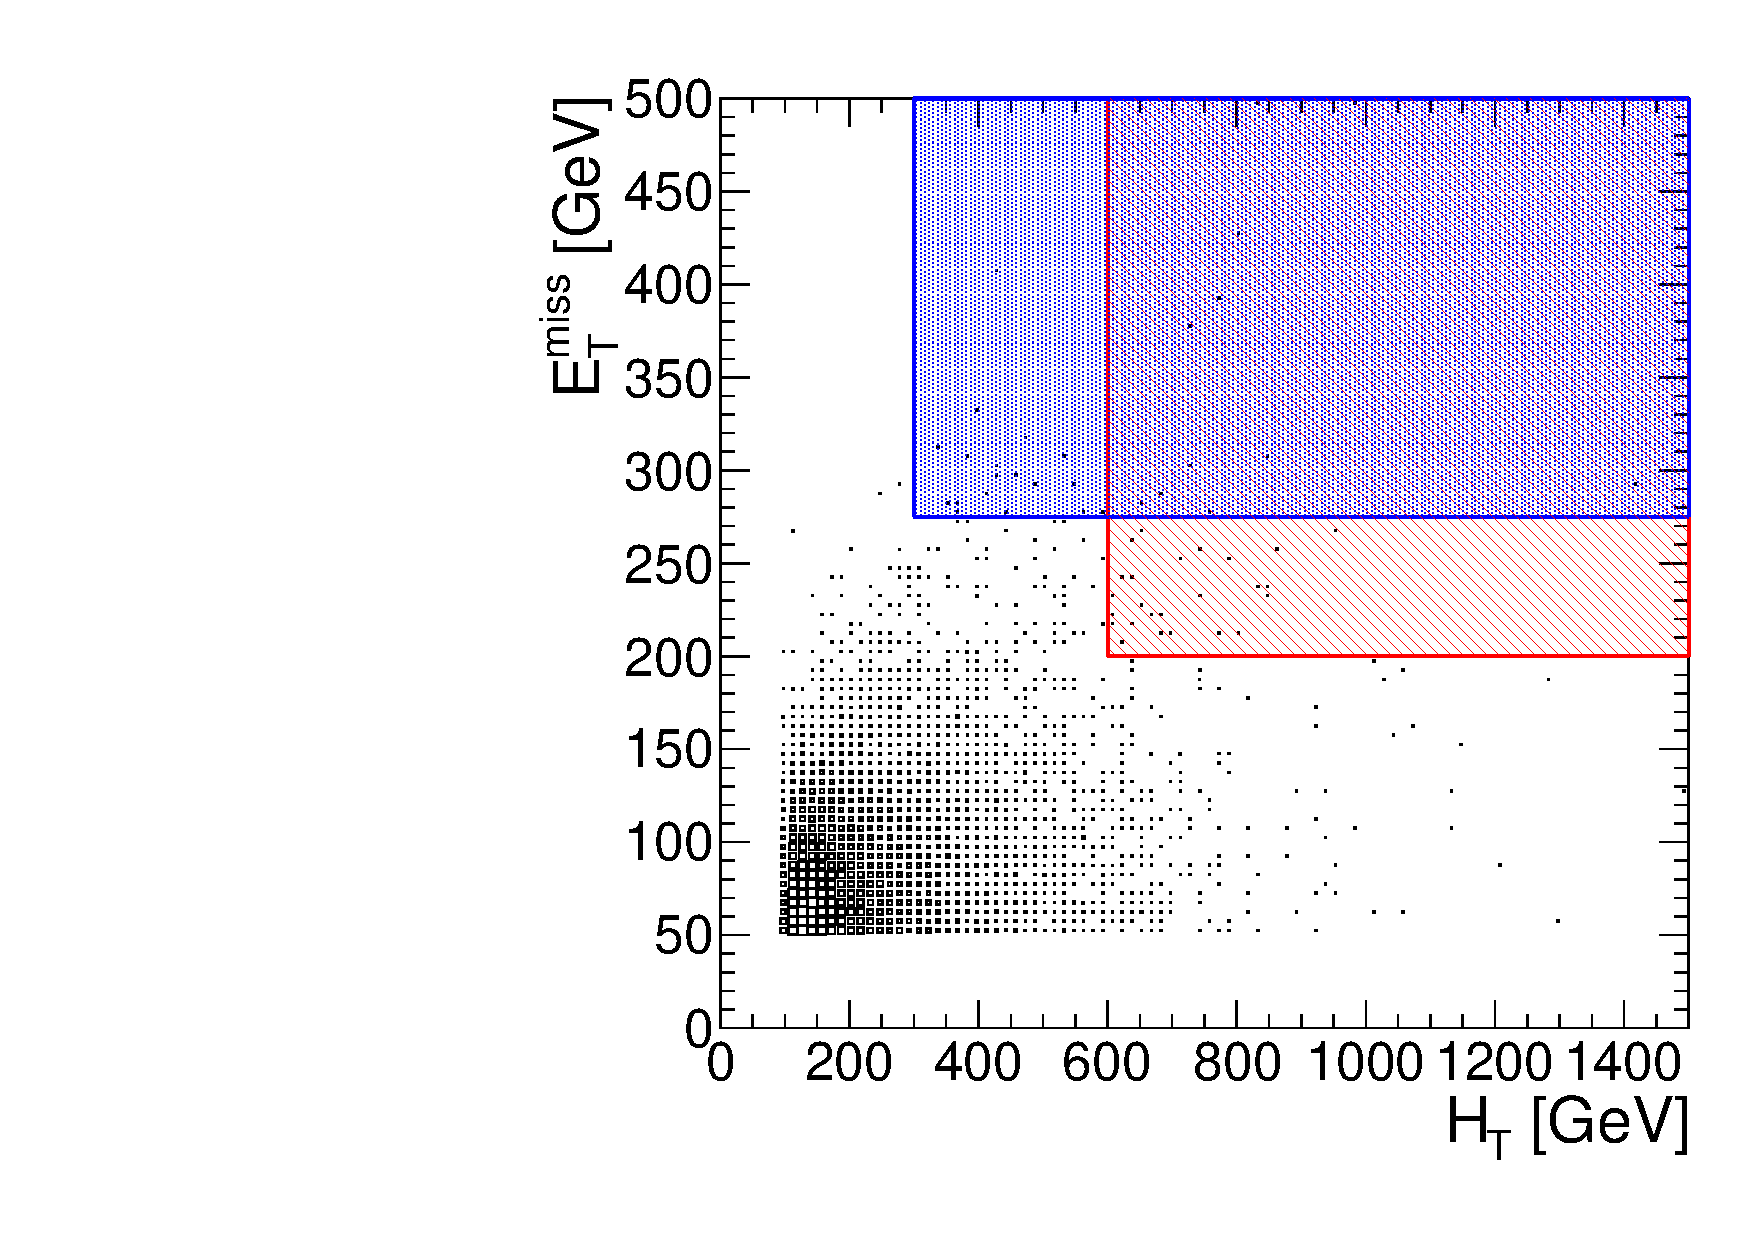
\includegraphics[width=0.45\linewidth]{plots/sigregions_met_ht_tt.pdf}
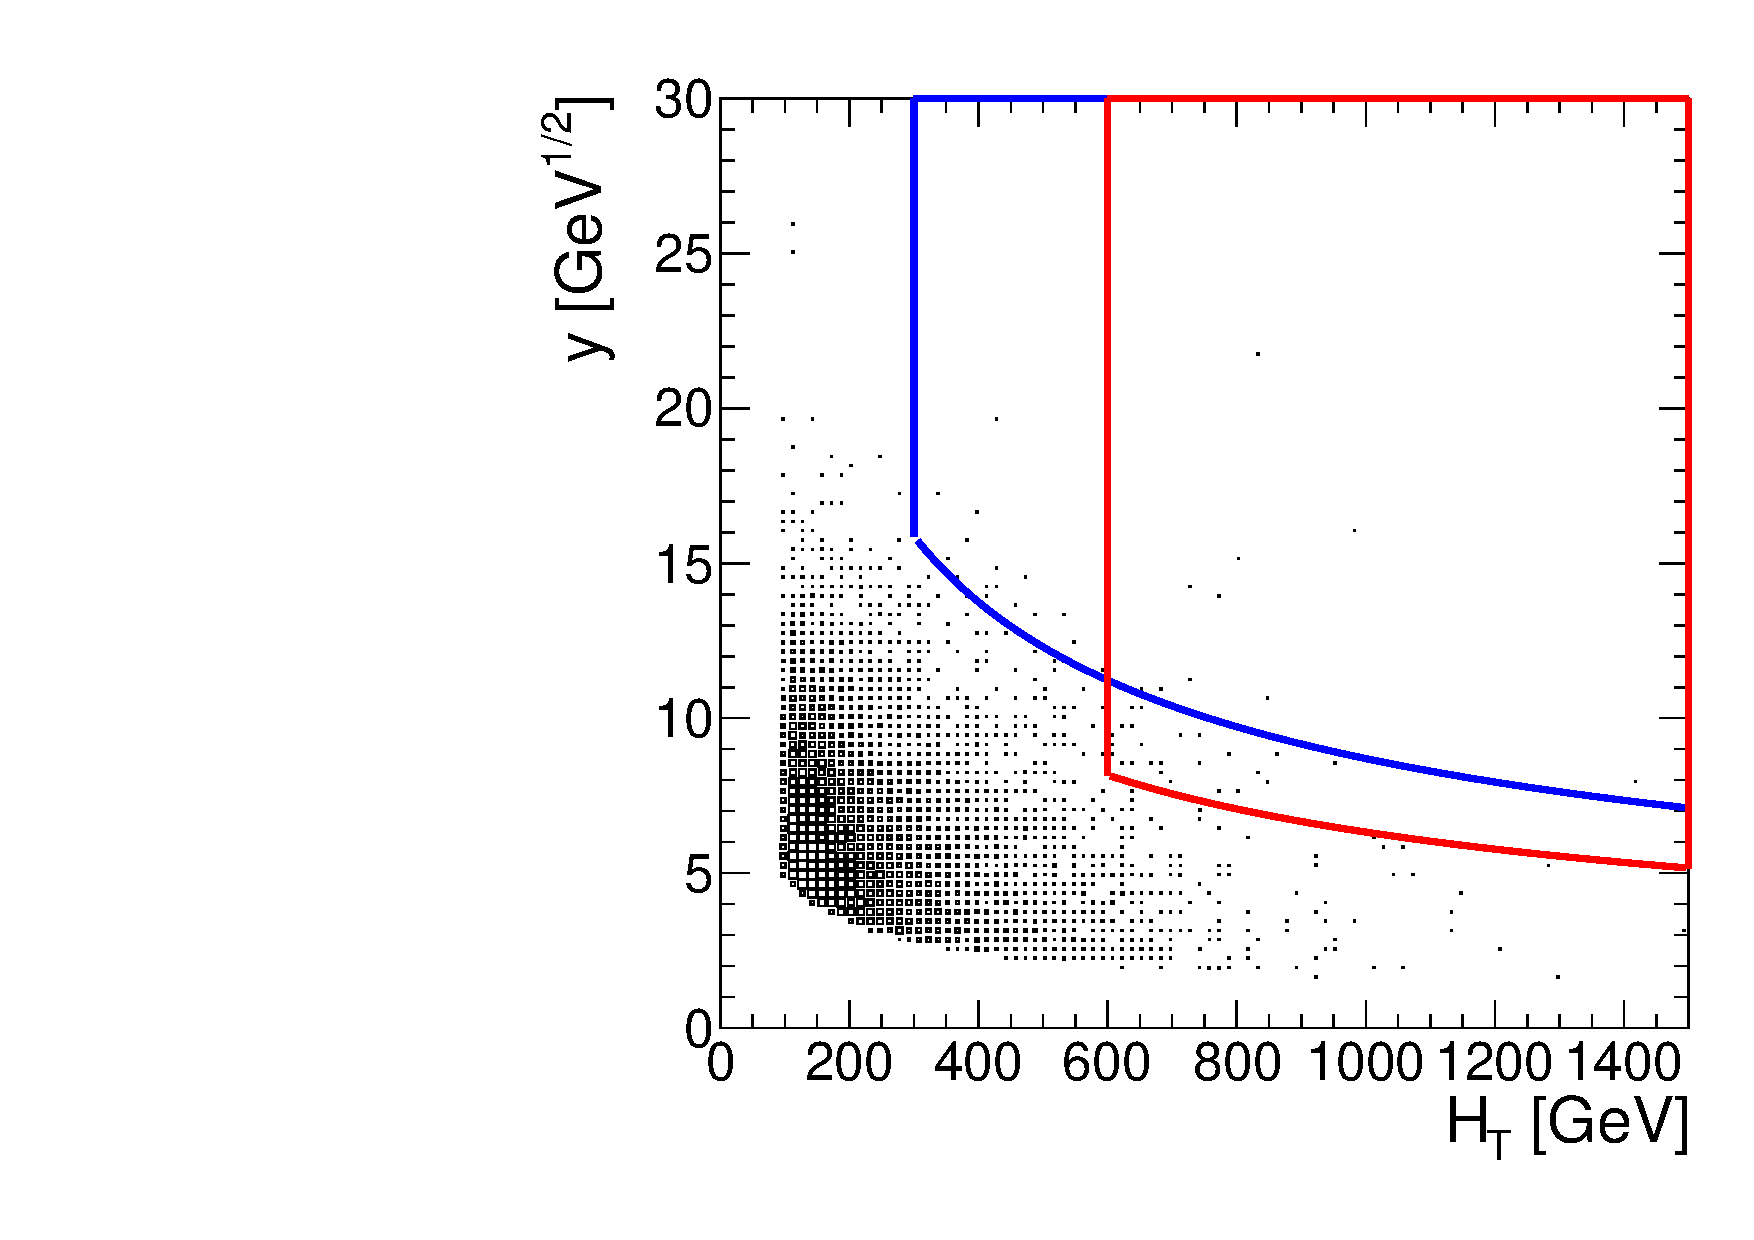
\includegraphics[width=0.45\linewidth]{plots/sigregions_y_ht_tt.pdf}
\caption{\label{fig:sigRegion}\protect
Illustration of signal regions for the 2011 analysis; \ttbar \, MC is plotted.
Left: \met\ vs. \Ht. The high \met\ signal region ( \met\ $>$ 275 GeV, \Ht\ $>$ 300 GeV)
is shown in blue. The high \Ht\ signal region ( \met\ $>$ 200 GeV, \Ht\ $>$ 600 GeV) is
shown in red. Right: The 2011 signal regions shown on the left are represented in
the $y$ vs. \Ht\ plane.
}
\end{center}
\end{figure}


Data yields are compared against Monte Carlo expectations in the following tables:

\begin{itemize}
  \item High \pt\ dilepton trigger sample:
    \begin{itemize}
      \item Table ~\ref{tab:sigyield1}: 2010 signal region
      \item Table ~\ref{tab:sigyield2}: 2011 high \met signal region
      \item Table ~\ref{tab:sigyield3}: 2011 high \Ht signal region
    \end{itemize}
  \item Dilepton-\Ht\ cross trigger sample ( events with \pt $>$ (20,10) are excluded ):
    \begin{itemize}
         \item Table \ref{tab:lowptsigyield1}: 2010 signal region
         \item Table \ref{tab:lowptsigyield2}: 2011 high \met signal region
         \item Table \ref{tab:lowptsigyield3}: 2011 high \Ht signal region
    \end{itemize}
\end{itemize}

Yields for the 2010 signal regions are presented in tables ~\ref{tab:sigyield1} and \ref{tab:lowptsigyield1}
to ensure that results from the 2011 analysis are consistent with the 2010 results.

\clearpage
%\newpage

\begin{table}[h!]
\begin{center}
\footnotesize
\caption{\label{tab:sigyield1} High \pt\ dilepton trigger data and MC yields in the 2010 signal region. 
MC errors are statistical only.
}
\vspace{.25cm}
\begin{tabular}{l|cccc}
\hline
         Sample   &           $ee$   &       $\mu\mu$   &         $e\mu$   &            tot  \\
\hline
           \ttll   &  4.4 $\pm$ 0.9   &  6.9 $\pm$ 1.1   & 12.6 $\pm$ 1.5   & 23.9 $\pm$ 2.1  \\
          \tttau   &  1.9 $\pm$ 0.6   &  2.0 $\pm$ 0.6   &  5.6 $\pm$ 1.0   &  9.5 $\pm$ 1.3  \\
         \ttfake   &  0.5 $\pm$ 0.3   &  0.0 $\pm$ 0.0   &  0.7 $\pm$ 0.4   &  1.2 $\pm$ 0.5  \\
              DY   &  0.9 $\pm$ 0.9   &  1.9 $\pm$ 1.9   &  2.0 $\pm$ 2.0   &  4.8 $\pm$ 2.9  \\
             \WW   &  0.2 $\pm$ 0.1   &  0.2 $\pm$ 0.1   &  0.4 $\pm$ 0.1   &  0.8 $\pm$ 0.2  \\
             \WZ   &  0.0 $\pm$ 0.0   &  0.0 $\pm$ 0.0   &  0.1 $\pm$ 0.0   &  0.1 $\pm$ 0.0  \\
             \ZZ   &  0.0 $\pm$ 0.0   &  0.0 $\pm$ 0.0   &  0.0 $\pm$ 0.0   &  0.1 $\pm$ 0.0  \\
      single top   &  0.2 $\pm$ 0.1   &  0.0 $\pm$ 0.0   &  0.1 $\pm$ 0.1   &  0.3 $\pm$ 0.1  \\
          \wjets   &  0.0 $\pm$ 0.0   &  0.0 $\pm$ 0.0   &  0.0 $\pm$ 0.0   &  0.0 $\pm$ 0.0  \\
\hline
      tot SM MC   &  8.1 $\pm$ 1.4   & 11.1 $\pm$ 2.3   & 21.5 $\pm$ 2.7   & 40.7 $\pm$ 3.8  \\
\hline
           data   &             11   &              8   &             26   &             45  \\
\hline
            LM1   & 30.7 $\pm$ 1.1   & 36.4 $\pm$ 1.2   & 18.6 $\pm$ 0.9   & 85.7 $\pm$ 1.9  \\
            LM3   &  8.9 $\pm$ 0.5   & 10.8 $\pm$ 0.6   & 15.0 $\pm$ 0.7   & 34.6 $\pm$ 1.0  \\
            LM6   &  2.9 $\pm$ 0.1   &  3.2 $\pm$ 0.1   &  3.7 $\pm$ 0.1   &  9.7 $\pm$ 0.2  \\
\hline
\end{tabular}
\end{center}
\end{table}


\begin{table}[h!]
\begin{center}
\footnotesize
\caption{\label{tab:sigyield2} High \pt\ dilepton trigger data and MC yields in the high \met\ signal region. MC errors are statistical only.}
\vspace{.25cm}
\begin{tabular}{l|cccc}
\hline
         Sample   &           $ee$   &       $\mu\mu$   &         $e\mu$   &            tot  \\
\hline
          \ttll   &  1.2 $\pm$ 0.5   &  1.0 $\pm$ 0.4   &  2.2 $\pm$ 0.7   &  4.3 $\pm$ 0.9  \\
         \tttau   &  0.3 $\pm$ 0.2   &  0.0 $\pm$ 0.0   &  0.4 $\pm$ 0.3   &  0.7 $\pm$ 0.4  \\
        \ttfake   &  0.0 $\pm$ 0.0   &  0.0 $\pm$ 0.0   &  0.0 $\pm$ 0.0   &  0.0 $\pm$ 0.0  \\
             DY   &  0.0 $\pm$ 0.0   &  0.0 $\pm$ 0.0   &  2.0 $\pm$ 2.0   &  2.0 $\pm$ 2.0  \\
            \WW   &  0.1 $\pm$ 0.1   &  0.1 $\pm$ 0.1   &  0.0 $\pm$ 0.0   &  0.2 $\pm$ 0.1  \\
            \WZ   &  0.0 $\pm$ 0.0   &  0.0 $\pm$ 0.0   &  0.0 $\pm$ 0.0   &  0.0 $\pm$ 0.0  \\
            \ZZ   &  0.0 $\pm$ 0.0   &  0.0 $\pm$ 0.0   &  0.0 $\pm$ 0.0   &  0.0 $\pm$ 0.0  \\
              t   &  0.0 $\pm$ 0.0   &  0.0 $\pm$ 0.0   &  0.0 $\pm$ 0.0   &  0.0 $\pm$ 0.0  \\
         \wjets   &  0.0 $\pm$ 0.0   &  0.0 $\pm$ 0.0   &  0.0 $\pm$ 0.0   &  0.0 $\pm$ 0.0  \\
\hline
      tot SM MC   &  1.6 $\pm$ 0.6   &  1.1 $\pm$ 0.4   &  4.6 $\pm$ 2.1   &  7.3 $\pm$ 2.2  \\
\hline
           data   &              5   &              0   &              3   &              8  \\
\hline
            LM1   & 17.5 $\pm$ 0.9   & 20.3 $\pm$ 0.9   & 10.9 $\pm$ 0.7   & 48.7 $\pm$ 1.4  \\
            LM3   &  4.8 $\pm$ 0.4   &  5.8 $\pm$ 0.4   &  7.4 $\pm$ 0.5   & 18.0 $\pm$ 0.7  \\
            LM6   &  2.4 $\pm$ 0.1   &  2.6 $\pm$ 0.1   &  3.0 $\pm$ 0.1   &  8.1 $\pm$ 0.2  \\
\hline
\end{tabular}
\end{center}
\end{table}

\begin{table}[h!]
\begin{center}
\footnotesize
\caption{\label{tab:sigyield3} High \pt\ dilepton trigger data and MC yields in the high \Ht\ signal region. MC errors are statistical only.}
\vspace{.25cm}
\begin{tabular}{l|cccc}
\hline
         Sample   &           $ee$   &       $\mu\mu$   &         $e\mu$   &            tot  \\
\hline
          \ttll   &  0.4 $\pm$ 0.3   &  0.9 $\pm$ 0.4   &  1.8 $\pm$ 0.6   &  3.2 $\pm$ 0.8  \\
         \tttau   &  0.3 $\pm$ 0.2   &  0.5 $\pm$ 0.3   &  1.0 $\pm$ 0.4   &  1.9 $\pm$ 0.6  \\
        \ttfake   &  0.0 $\pm$ 0.0   &  0.0 $\pm$ 0.0   &  0.0 $\pm$ 0.0   &  0.0 $\pm$ 0.0  \\
             DY   &  0.0 $\pm$ 0.0   &  0.0 $\pm$ 0.0   &  2.0 $\pm$ 2.0   &  2.0 $\pm$ 2.0  \\
            \WW   &  0.0 $\pm$ 0.0   &  0.0 $\pm$ 0.0   &  0.0 $\pm$ 0.0   &  0.0 $\pm$ 0.0  \\
            \WZ   &  0.0 $\pm$ 0.0   &  0.0 $\pm$ 0.0   &  0.0 $\pm$ 0.0   &  0.0 $\pm$ 0.0  \\
            \ZZ   &  0.0 $\pm$ 0.0   &  0.0 $\pm$ 0.0   &  0.0 $\pm$ 0.0   &  0.0 $\pm$ 0.0  \\
     single top   &  0.0 $\pm$ 0.0   &  0.0 $\pm$ 0.0   &  0.0 $\pm$ 0.0   &  0.0 $\pm$ 0.0  \\
         \wjets   &  0.0 $\pm$ 0.0   &  0.0 $\pm$ 0.0   &  0.0 $\pm$ 0.0   &  0.0 $\pm$ 0.0  \\
\hline
      tot SM MC   &  0.7 $\pm$ 0.4   &  1.5 $\pm$ 0.5   &  4.9 $\pm$ 2.1   &  7.1 $\pm$ 2.2  \\
\hline
           data   &              1   &              0   &              3   &              4  \\
\hline
            LM1   & 14.9 $\pm$ 0.8   & 15.9 $\pm$ 0.8   &  7.0 $\pm$ 0.5   & 37.7 $\pm$ 1.3  \\
            LM3   &  5.2 $\pm$ 0.4   &  5.8 $\pm$ 0.4   &  7.7 $\pm$ 0.5   & 18.8 $\pm$ 0.8  \\
            LM6   &  2.2 $\pm$ 0.1   &  2.5 $\pm$ 0.1   &  2.7 $\pm$ 0.1   &  7.4 $\pm$ 0.1  \\
\hline
\end{tabular}
\end{center}
\end{table}


\clearpage
%\newpage

\begin{table}[h!]
\begin{center}
\footnotesize
\caption{\label{tab:lowptsigyield1} Dilepton-\Ht trigger data and MC yields in the 2010 signal region. MC errors are statistical only.
}
\vspace{.25cm}
\begin{tabular}{l|cccc}
\hline
         Sample   &           $ee$   &       $\mu\mu$   &         $e\mu$   &            tot  \\
\hline
          \ttll   &  0.0 $\pm$ 0.0   &  0.4 $\pm$ 0.3   &  1.1 $\pm$ 0.5   &  1.5 $\pm$ 0.5  \\
         \tttau   &  0.0 $\pm$ 0.0   &  0.6 $\pm$ 0.3   &  0.2 $\pm$ 0.2   &  0.8 $\pm$ 0.4  \\
        \ttfake   &  0.0 $\pm$ 0.0   &  0.0 $\pm$ 0.0   &  0.3 $\pm$ 0.2   &  0.3 $\pm$ 0.2  \\
             DY   &  0.0 $\pm$ 0.0   &  0.0 $\pm$ 0.0   &  0.0 $\pm$ 0.0   &  0.0 $\pm$ 0.0  \\
            \WW   &  0.0 $\pm$ 0.0   &  0.0 $\pm$ 0.0   &  0.0 $\pm$ 0.0   &  0.0 $\pm$ 0.0  \\
            \WZ   &  0.0 $\pm$ 0.0   &  0.0 $\pm$ 0.0   &  0.0 $\pm$ 0.0   &  0.0 $\pm$ 0.0  \\
            \ZZ   &  0.0 $\pm$ 0.0   &  0.0 $\pm$ 0.0   &  0.0 $\pm$ 0.0   &  0.0 $\pm$ 0.0  \\
     single top   &  0.0 $\pm$ 0.0   &  0.0 $\pm$ 0.0   &  0.0 $\pm$ 0.0   &  0.0 $\pm$ 0.0  \\
         \wjets   &  0.0 $\pm$ 0.0   &  0.0 $\pm$ 0.0   &  0.0 $\pm$ 0.0   &  0.0 $\pm$ 0.0  \\
\hline
      tot SM MC   &  0.0 $\pm$ 0.0   &  1.1 $\pm$ 0.4   &  1.6 $\pm$ 0.5   &  2.7 $\pm$ 0.7  \\
\hline
           data   &              0   &              2   &              2   &              4  \\
\hline
            LM1   &  0.8 $\pm$ 0.2   &  7.4 $\pm$ 0.5   &  5.9 $\pm$ 0.5   & 14.2 $\pm$ 0.8  \\
            LM3   &  0.1 $\pm$ 0.0   &  1.2 $\pm$ 0.2   &  1.0 $\pm$ 0.2   &  2.2 $\pm$ 0.3  \\
            LM6   &  0.0 $\pm$ 0.0   &  0.3 $\pm$ 0.0   &  0.2 $\pm$ 0.0   &  0.5 $\pm$ 0.0  \\
\hline
\end{tabular}
\end{center}
\end{table}


\begin{table}[h!]
\begin{center}
\footnotesize
\caption{\label{tab:lowptsigyield2} Dilepton-\Ht\ trigger data and MC yields in the high \met\ signal region.
MC errors are statistical only.
}
\vspace{.25cm}
\begin{tabular}{l|cccc}
\hline
         Sample   &           $ee$   &       $\mu\mu$   &         $e\mu$   &            tot  \\
\hline
          \ttll   &  0.0 $\pm$ 0.0   &  0.1 $\pm$ 0.1   &  0.0 $\pm$ 0.0   &  0.1 $\pm$ 0.1  \\
         \tttau   &  0.0 $\pm$ 0.0   &  0.0 $\pm$ 0.0   &  0.2 $\pm$ 0.2   &  0.2 $\pm$ 0.2  \\
        \ttfake   &  0.0 $\pm$ 0.0   &  0.0 $\pm$ 0.0   &  0.0 $\pm$ 0.0   &  0.0 $\pm$ 0.0  \\
             DY   &  0.0 $\pm$ 0.0   &  0.0 $\pm$ 0.0   &  0.0 $\pm$ 0.0   &  0.0 $\pm$ 0.0  \\
            \WW   &  0.0 $\pm$ 0.0   &  0.0 $\pm$ 0.0   &  0.0 $\pm$ 0.0   &  0.0 $\pm$ 0.0  \\
            \WZ   &  0.0 $\pm$ 0.0   &  0.0 $\pm$ 0.0   &  0.0 $\pm$ 0.0   &  0.0 $\pm$ 0.0  \\
            \ZZ   &  0.0 $\pm$ 0.0   &  0.0 $\pm$ 0.0   &  0.0 $\pm$ 0.0   &  0.0 $\pm$ 0.0  \\
     single top   &  0.0 $\pm$ 0.0   &  0.0 $\pm$ 0.0   &  0.0 $\pm$ 0.0   &  0.0 $\pm$ 0.0  \\
         \wjets   &  0.0 $\pm$ 0.0   &  0.0 $\pm$ 0.0   &  0.0 $\pm$ 0.0   &  0.0 $\pm$ 0.0  \\
\hline
      tot SM MC   &  0.0 $\pm$ 0.0   &  0.1 $\pm$ 0.1   &  0.2 $\pm$ 0.2   &  0.3 $\pm$ 0.2  \\
\hline
           data   &              0   &              0   &              0   &              0  \\
\hline
            LM1   &  0.4 $\pm$ 0.1   &  4.4 $\pm$ 0.4   &  3.5 $\pm$ 0.4   &  8.3 $\pm$ 0.6  \\
            LM3   &  0.1 $\pm$ 0.0   &  0.7 $\pm$ 0.1   &  0.6 $\pm$ 0.1   &  1.3 $\pm$ 0.2  \\
            LM6   &  0.0 $\pm$ 0.0   &  0.3 $\pm$ 0.0   &  0.1 $\pm$ 0.0   &  0.4 $\pm$ 0.0  \\
\hline
\end{tabular}
\end{center}
\end{table}

\begin{table}[h!]
\begin{center}
\footnotesize
\caption{\label{tab:lowptsigyield3} Dilepton-\Ht\ trigger data and MC yields in the high \Ht\ signal region.
MC errors are statistical only.
}
\vspace{.25cm}
\begin{tabular}{l|cccc}
\hline
         Sample   &           $ee$   &       $\mu\mu$   &         $e\mu$   &            tot  \\
\hline
          \ttll   &  0.0 $\pm$ 0.0   &  0.0 $\pm$ 0.0   &  0.0 $\pm$ 0.0   &  0.0 $\pm$ 0.0  \\
         \tttau   &  0.0 $\pm$ 0.0   &  0.0 $\pm$ 0.0   &  0.0 $\pm$ 0.0   &  0.0 $\pm$ 0.0  \\
        \ttfake   &  0.0 $\pm$ 0.0   &  0.0 $\pm$ 0.0   &  0.0 $\pm$ 0.0   &  0.0 $\pm$ 0.0  \\
             DY   &  0.0 $\pm$ 0.0   &  0.0 $\pm$ 0.0   &  0.0 $\pm$ 0.0   &  0.0 $\pm$ 0.0  \\
            \WW   &  0.0 $\pm$ 0.0   &  0.0 $\pm$ 0.0   &  0.0 $\pm$ 0.0   &  0.0 $\pm$ 0.0  \\
            \WZ   &  0.0 $\pm$ 0.0   &  0.0 $\pm$ 0.0   &  0.0 $\pm$ 0.0   &  0.0 $\pm$ 0.0  \\
            \ZZ   &  0.0 $\pm$ 0.0   &  0.0 $\pm$ 0.0   &  0.0 $\pm$ 0.0   &  0.0 $\pm$ 0.0  \\
     single top   &  0.0 $\pm$ 0.0   &  0.0 $\pm$ 0.0   &  0.0 $\pm$ 0.0   &  0.0 $\pm$ 0.0  \\
         \wjets   &  0.0 $\pm$ 0.0   &  0.0 $\pm$ 0.0   &  0.0 $\pm$ 0.0   &  0.0 $\pm$ 0.0  \\
\hline
      tot SM MC   &  0.0 $\pm$ 0.0   &  0.1 $\pm$ 0.0   &  0.0 $\pm$ 0.0   &  0.1 $\pm$ 0.0  \\
\hline
           data   &              0   &              0   &              1   &              1  \\
\hline
            LM1   &  0.4 $\pm$ 0.1   &  3.8 $\pm$ 0.4   &  2.1 $\pm$ 0.3   &  6.3 $\pm$ 0.5  \\
            LM3   &  0.1 $\pm$ 0.1   &  0.8 $\pm$ 0.2   &  0.4 $\pm$ 0.1   &  1.3 $\pm$ 0.2  \\
            LM6   &  0.0 $\pm$ 0.0   &  0.3 $\pm$ 0.0   &  0.1 $\pm$ 0.0   &  0.4 $\pm$ 0.0  \\
\hline
\end{tabular}
\end{center}
\end{table}

\clearpage
%\newpage

These results are summarized as:

\begin{itemize}
\item High \pt\ dilepton trigger sample
\begin{itemize}
\item 2010 signal region ($y >$ 8.5 GeV$^{1/2}$, \Ht\ $>$ 300 GeV)
   \begin{itemize} 
   \item observed yield : 45 
   \item MC prediction  : $40.7 \pm 3.8$
   \end{itemize}  
\item high \met\ signal region (\met\ $>$ 275 GeV, \Ht\ $>$ 300 GeV)
   \begin{itemize} 
   \item observed yield : 8 
   \item MC prediction  : $7.3 \pm 2.2$
   \end{itemize}  
\item high \Ht\ signal region (\met\ $>$ 200 GeV, \Ht\ $>$ 600 GeV)
   \begin{itemize} 
   \item observed yield : 4 
   \item MC prediction  : $7.1 \pm 2.2$
   \end{itemize}  
\end{itemize}

\item Dilepton-\Ht\ trigger sample ( events with \pt $>$ (20,10) are excluded)
\begin{itemize}
\item 2010 signal region ($y >$ 8.5 GeV$^{1/2}$, \Ht\ $>$ 300 GeV)
   \begin{itemize} 
   \item observed yield : 4
   \item MC prediction  : $2.7 \pm 0.7$
   \end{itemize}  
\item high \met\ signal region (\met\ $>$ 275 GeV, \Ht\ $>$ 300 GeV)
   \begin{itemize} 
   \item observed yield : 0 
   \item MC prediction  : $0.3 \pm 0.2$
   \end{itemize}  
\item high \Ht\ signal region (\met\ $>$ 200 GeV, \Ht\ $>$ 600 GeV)
   \begin{itemize} 
   \item observed yield : 1 
   \item MC prediction  : $0.0 \pm 0.0$
   \end{itemize}  
\end{itemize}
\end{itemize}

For all signal regions, we observe reasonable agreement between data and MC expectations. 
A data/MC comparison of the kinematic distributions of the 45 events passing
the 2010 signal region selection is presented in App.~\ref{sec:appendix_datamc_sig}.

